\documentclass[letterpaper,12pt]{article}\usepackage[]{graphicx}\usepackage[]{color}
%% maxwidth is the original width if it is less than linewidth
%% otherwise use linewidth (to make sure the graphics do not exceed the margin)
\makeatletter
\def\maxwidth{ %
  \ifdim\Gin@nat@width>\linewidth
    \linewidth
  \else
    \Gin@nat@width
  \fi
}
\makeatother

\definecolor{fgcolor}{rgb}{0.345, 0.345, 0.345}
\newcommand{\hlnum}[1]{\textcolor[rgb]{0.686,0.059,0.569}{#1}}%
\newcommand{\hlstr}[1]{\textcolor[rgb]{0.192,0.494,0.8}{#1}}%
\newcommand{\hlcom}[1]{\textcolor[rgb]{0.678,0.584,0.686}{\textit{#1}}}%
\newcommand{\hlopt}[1]{\textcolor[rgb]{0,0,0}{#1}}%
\newcommand{\hlstd}[1]{\textcolor[rgb]{0.345,0.345,0.345}{#1}}%
\newcommand{\hlkwa}[1]{\textcolor[rgb]{0.161,0.373,0.58}{\textbf{#1}}}%
\newcommand{\hlkwb}[1]{\textcolor[rgb]{0.69,0.353,0.396}{#1}}%
\newcommand{\hlkwc}[1]{\textcolor[rgb]{0.333,0.667,0.333}{#1}}%
\newcommand{\hlkwd}[1]{\textcolor[rgb]{0.737,0.353,0.396}{\textbf{#1}}}%
\let\hlipl\hlkwb

\usepackage{framed}
\makeatletter
\newenvironment{kframe}{%
 \def\at@end@of@kframe{}%
 \ifinner\ifhmode%
  \def\at@end@of@kframe{\end{minipage}}%
  \begin{minipage}{\columnwidth}%
 \fi\fi%
 \def\FrameCommand##1{\hskip\@totalleftmargin \hskip-\fboxsep
 \colorbox{shadecolor}{##1}\hskip-\fboxsep
     % There is no \\@totalrightmargin, so:
     \hskip-\linewidth \hskip-\@totalleftmargin \hskip\columnwidth}%
 \MakeFramed {\advance\hsize-\width
   \@totalleftmargin\z@ \linewidth\hsize
   \@setminipage}}%
 {\par\unskip\endMakeFramed%
 \at@end@of@kframe}
\makeatother

\definecolor{shadecolor}{rgb}{.97, .97, .97}
\definecolor{messagecolor}{rgb}{0, 0, 0}
\definecolor{warningcolor}{rgb}{1, 0, 1}
\definecolor{errorcolor}{rgb}{1, 0, 0}
\newenvironment{knitrout}{}{} % an empty environment to be redefined in TeX

\usepackage{alltt}
\usepackage[top=1in,bottom=1in,left=1in,right=1in]{geometry}
\usepackage{setspace}
\usepackage[colorlinks=true,urlcolor=blue,citecolor=blue,linkcolor=blue]{hyperref}
\usepackage{indentfirst}
\usepackage{multirow}
\usepackage{booktabs}
\usepackage[final]{animate}
\usepackage{graphicx}
\usepackage{verbatim}
\usepackage{rotating}
\usepackage{tabularx}
\usepackage{array}
\usepackage{subfig} 
\usepackage[noae]{Sweave}
\usepackage{cleveref}
\usepackage[figureposition=bottom]{caption}
\usepackage{paralist}
\usepackage{acronym}
\usepackage{outlines}
\usepackage{pdflscape}

% knitr options


% housekeeping


\linespread{1}
\IfFileExists{upquote.sty}{\usepackage{upquote}}{}
\begin{document}

\begin{figure}
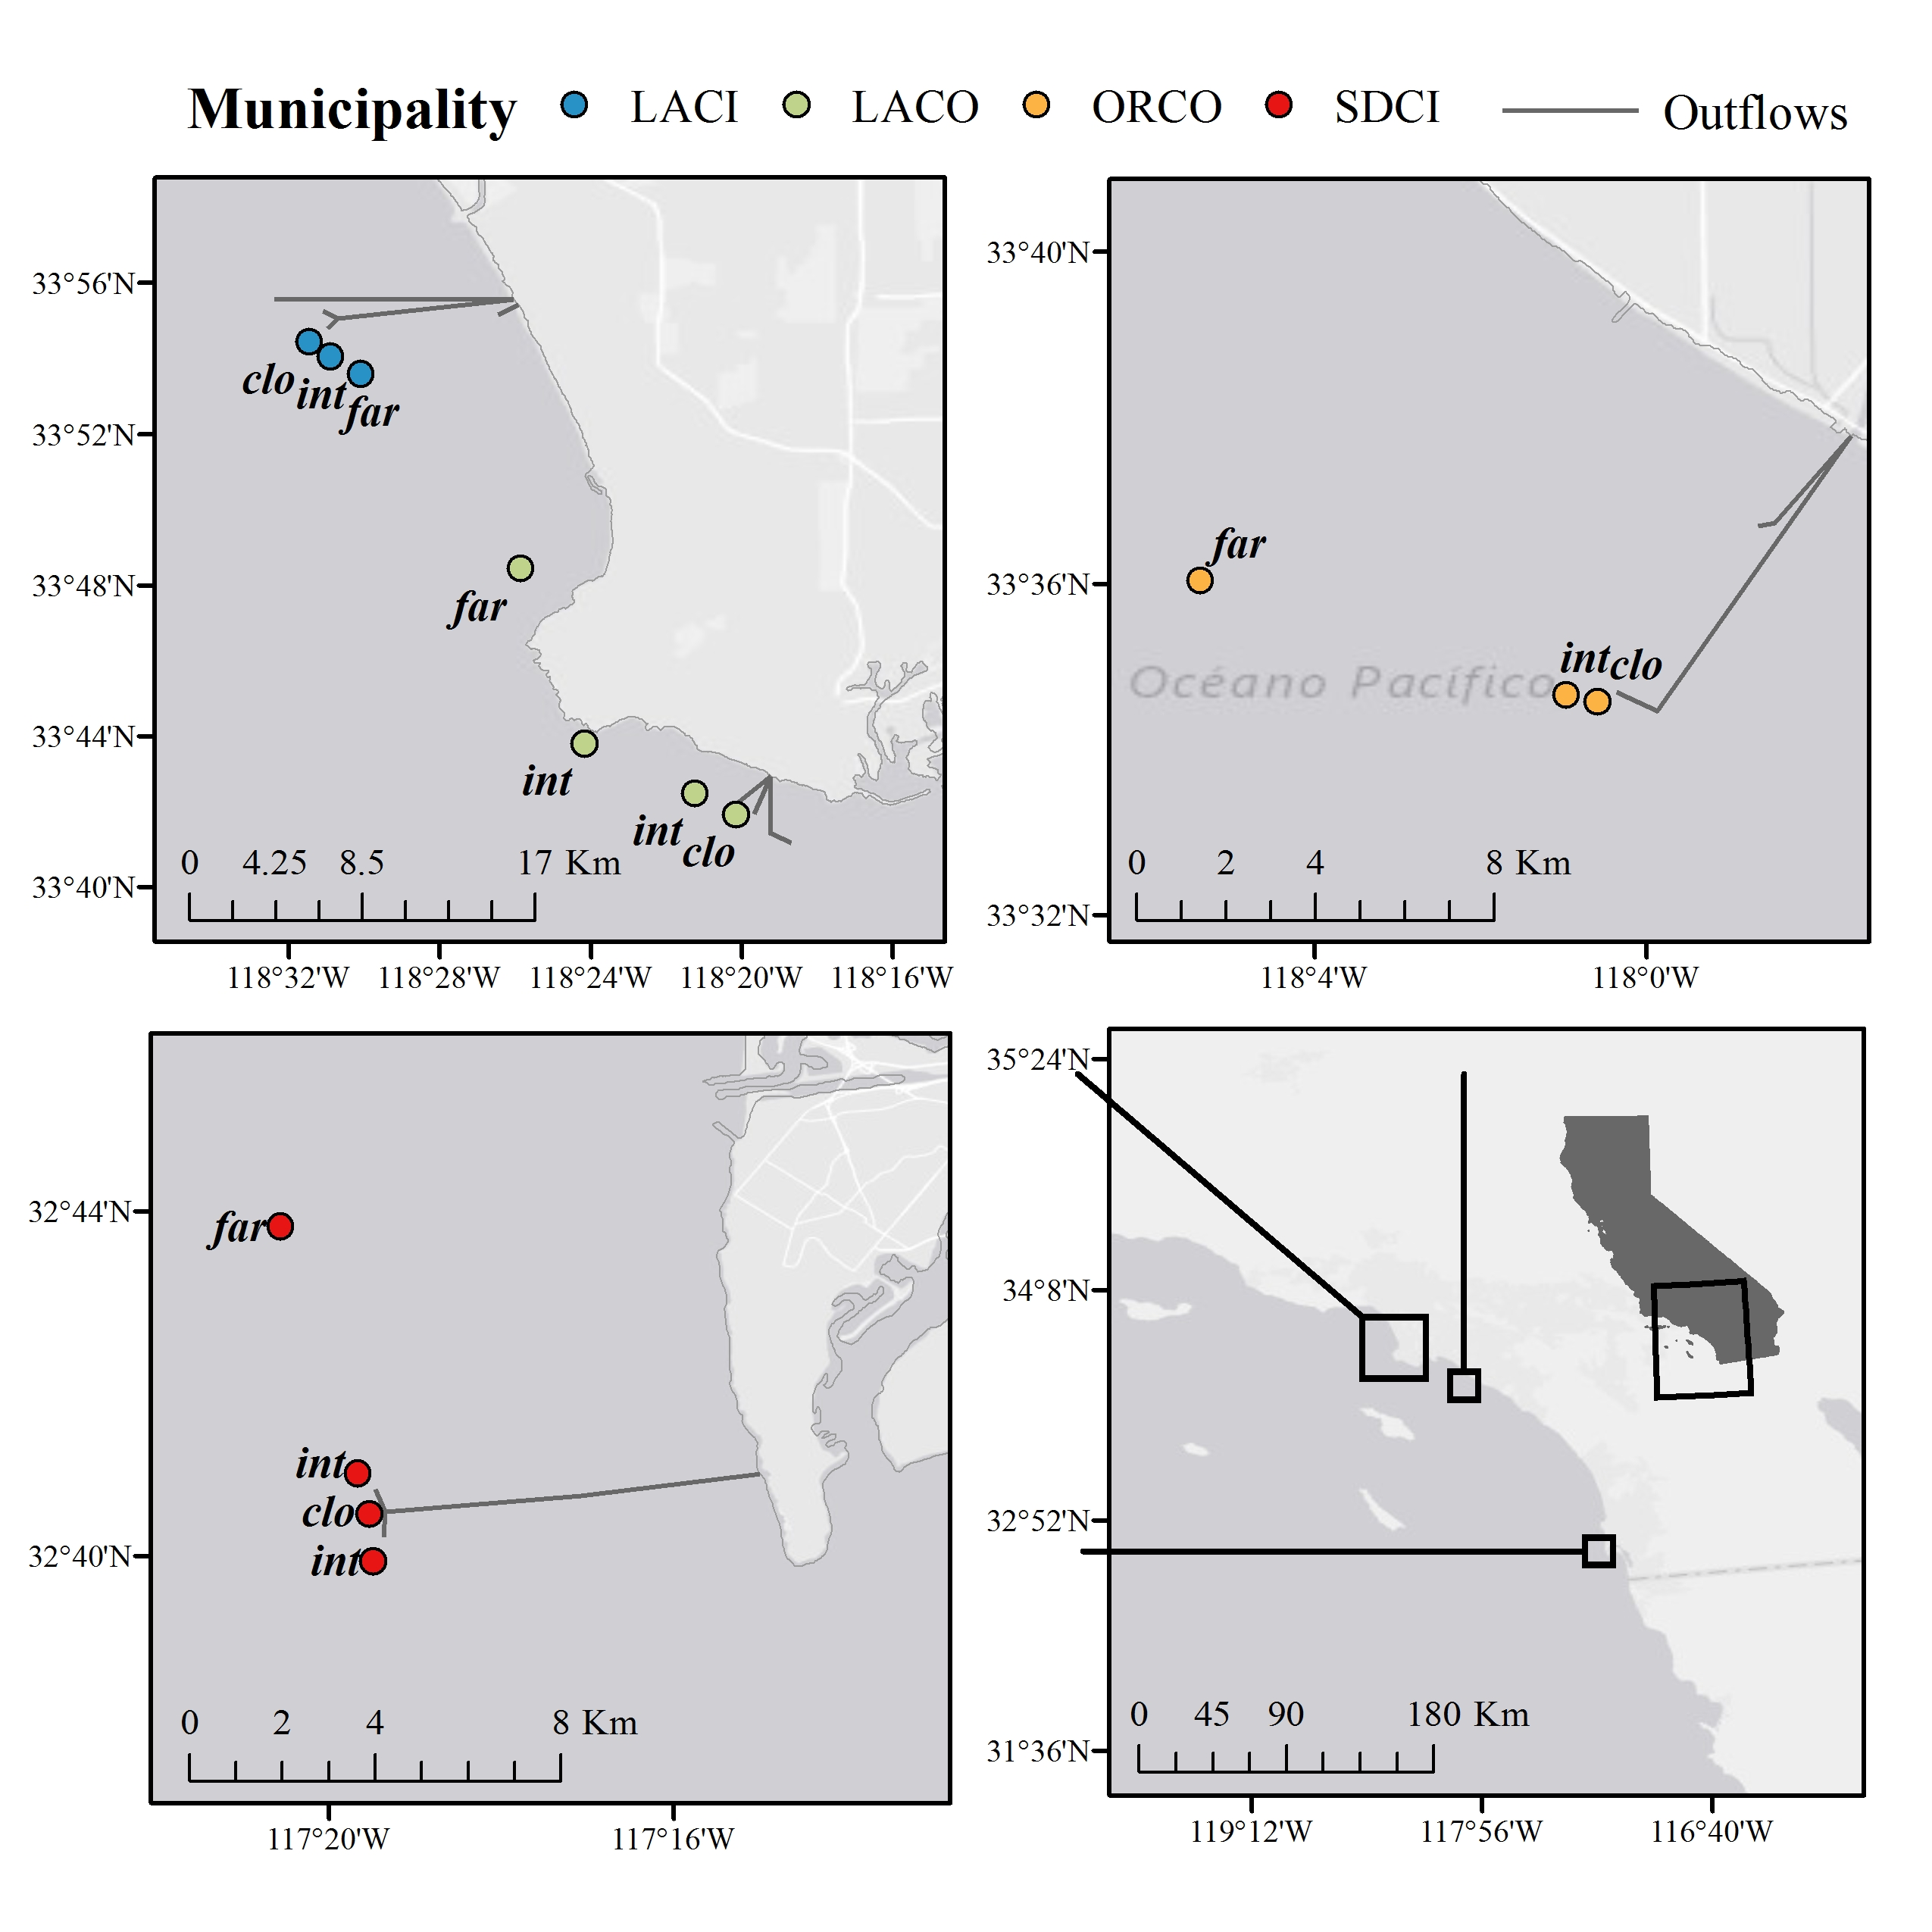
\includegraphics[width = \textwidth]{figs/sites.jpg}
\caption{Sampling stations grouped by municipality and approximate distance from wastewater treatment plant outflow pipes. Distances are close (clo), intermediate (int), and far. Municipalities are city of Los Angeles (LACI), city of San Diego (SDCI), Los Angeles County (LACO), and Orange County (ORCO).} 
\end{figure}



\begin{knitrout}
\definecolor{shadecolor}{rgb}{0.969, 0.969, 0.969}\color{fgcolor}\begin{figure}[!ht]

{\centering 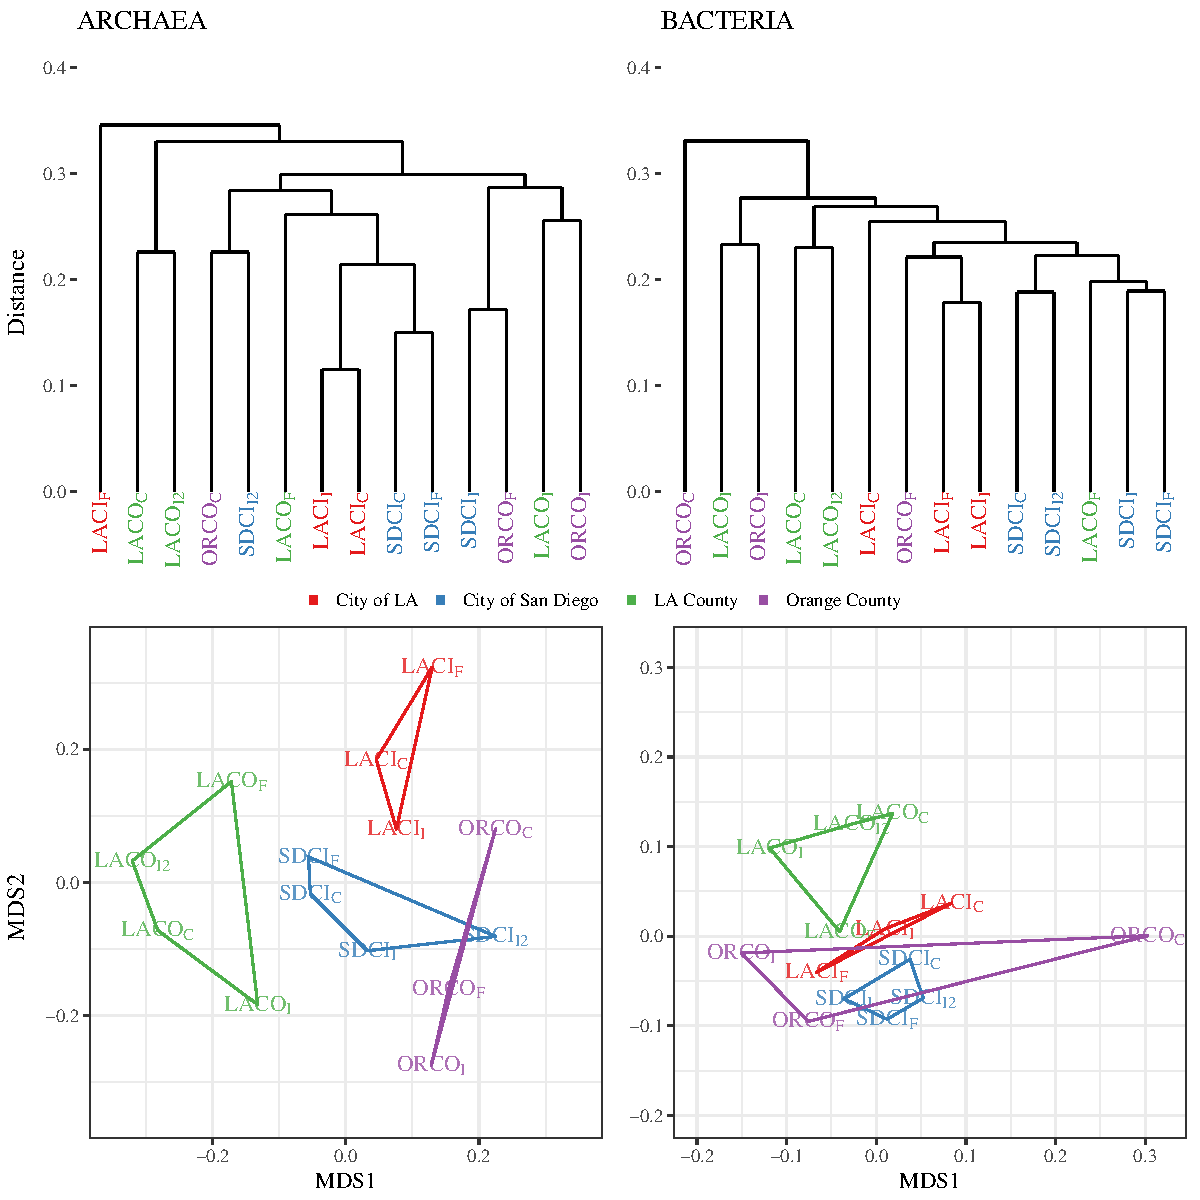
\includegraphics[width=\textwidth]{figs/clust1_arch} 

}

\caption[Site clusters and ordinations of microbial genera by domain]{Site clusters and ordinations of microbial genera by domain.  Colors indicate municipality and subscripts indicate distance categories from an outflow pipe at each site (`F' is farthest, `C' is closest, `I' is intermediate).  Clustering was based on a Bray-Curtis dissimilarity matrix of abundance data and sorting using the unweighted pair group method.  Ordinations were based on multi-dimensional scaling with two axes for the same data.  Abundance data were log-transformed prior to analysis. LACI: City of LA, SDCI: City of San Diego, LACO: LA County, ORCO: Orange County.}\label{fig:clust1_arch}
\end{figure}


\end{knitrout}

\begin{knitrout}
\definecolor{shadecolor}{rgb}{0.969, 0.969, 0.969}\color{fgcolor}\begin{figure}[!ht]

{\centering 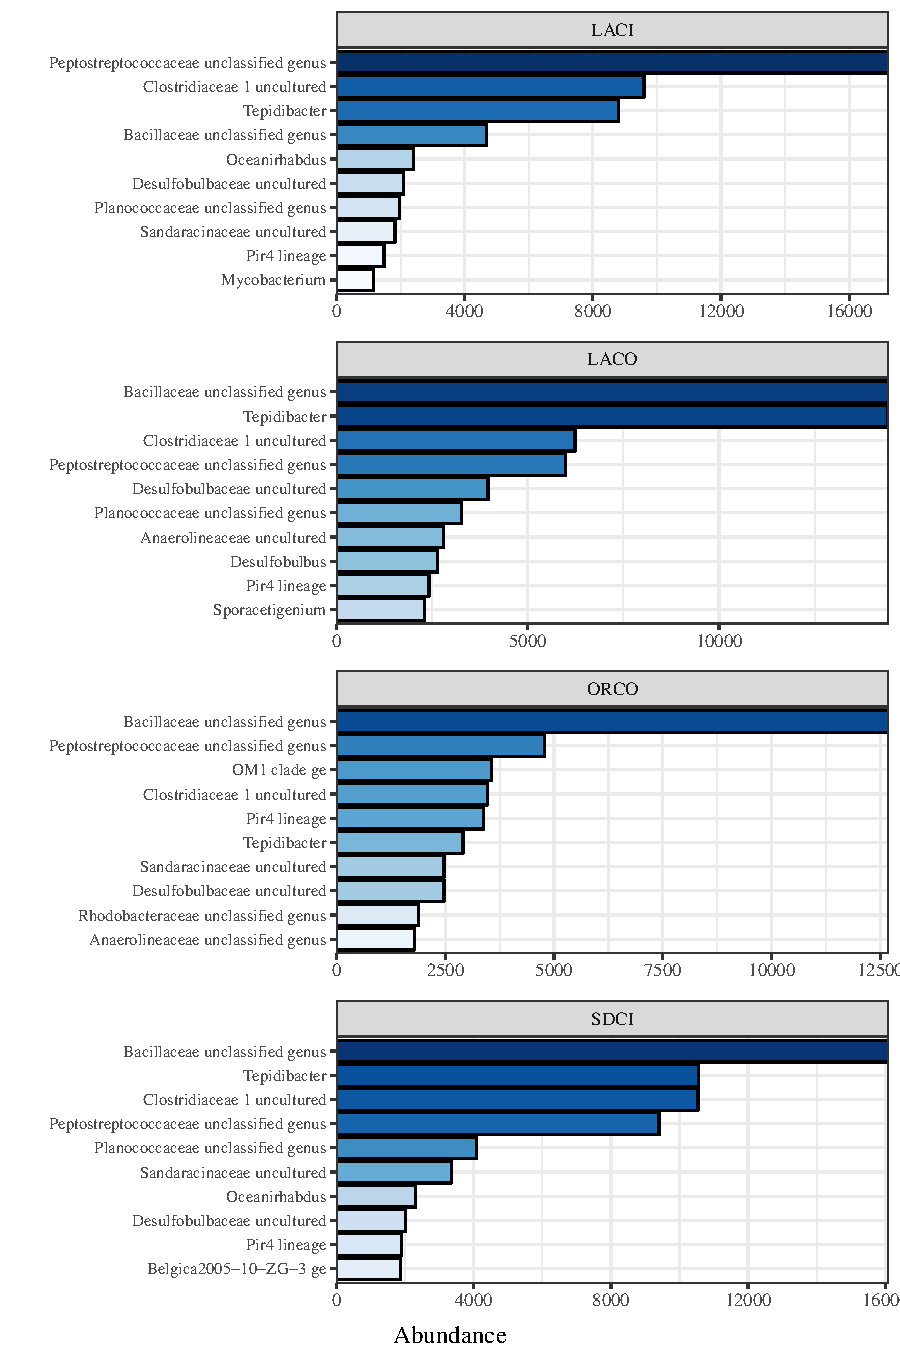
\includegraphics[width=\textwidth]{figs/abundwwtp} 

}

\caption[Top ten genera by OTU abundance grouped by domain and municipality of wastewater treatment plants]{Top ten genera by OTU abundance grouped by domain and municipality of wastewater treatment plants.}\label{fig:abundwwtp}
\end{figure}


\end{knitrout}
\clearpage

\begin{knitrout}
\definecolor{shadecolor}{rgb}{0.969, 0.969, 0.969}\color{fgcolor}\begin{figure}[!ht]

{\centering 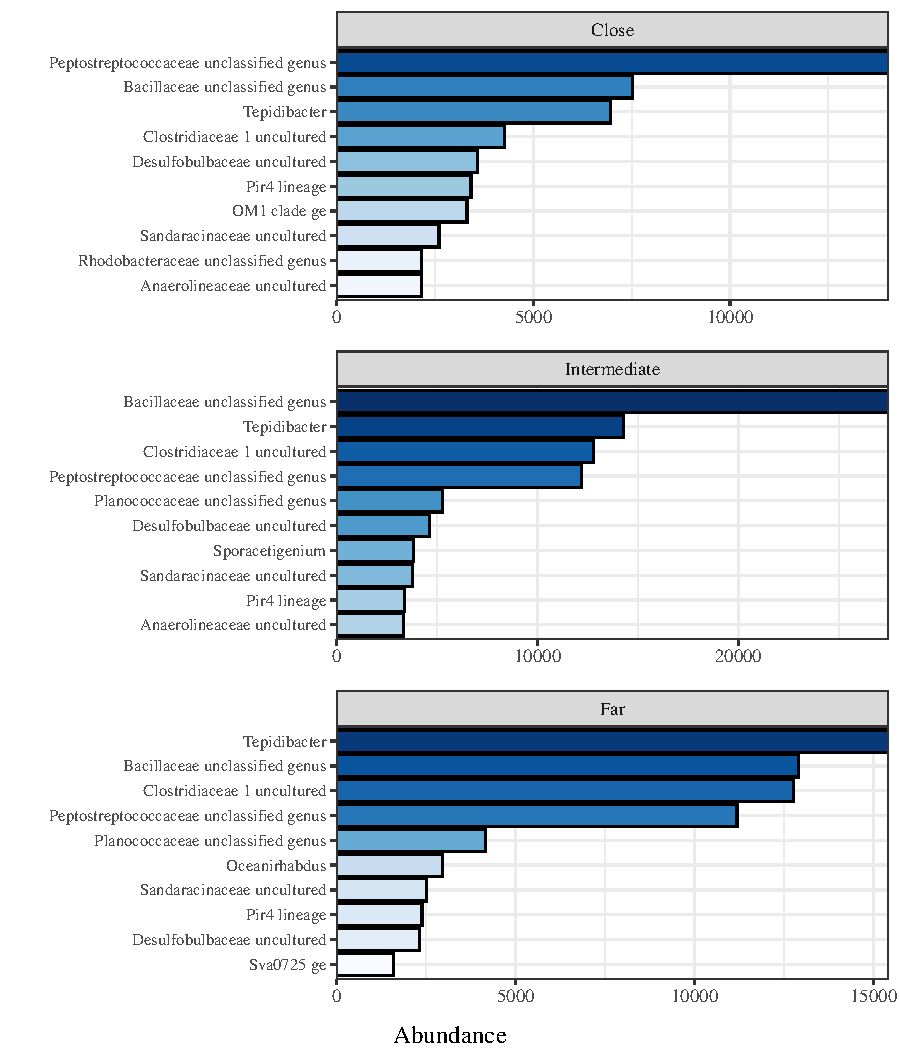
\includegraphics[width=\textwidth]{figs/abundcont} 

}

\caption[Top ten genera by OTU abundance grouped by approximate distance from wastewater treatment outflows]{Top ten genera by OTU abundance grouped by approximate distance from wastewater treatment outflows.}\label{fig:abundcont}
\end{figure}


\end{knitrout}
\clearpage

\clearpage
% ANOVA wwtp
\begin{knitrout}
\definecolor{shadecolor}{rgb}{0.969, 0.969, 0.969}\color{fgcolor}\begin{figure}[!ht]

{\centering 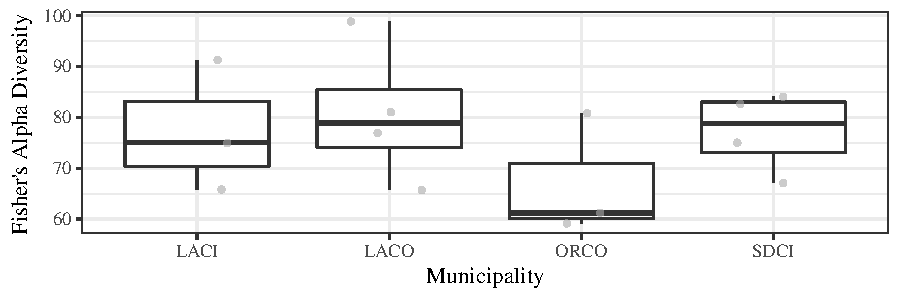
\includegraphics[width=\maxwidth]{figs/boxdivwwtp} 

}

\caption[Estimates of Fisher's alpha diversity for archaea and bacteria genera grouped by municipality of wastewater treatment plant]{Estimates of Fisher's alpha diversity for archaea and bacteria genera grouped by municipality of wastewater treatment plant. Alpha was was based on methods in Fisher et al. (1943) that measure diversity as a function of richness and abundance at a site.}\label{fig:boxdivwwtp}
\end{figure}


\end{knitrout}

% Table created by stargazer v.5.2 by Marek Hlavac, Harvard University. E-mail: hlavac at fas.harvard.edu
% Date and time: Fri, Nov 03, 2017 - 3:17:42 PM
\begin{table}[!htbp] \centering 
  \caption{Summary of analysis of variance results for bacteria and archaea diversity by municipality.  Diversity measures were based on Fisher's Alpha (Fisher et al. 1943) using abundance of genera at each site. The model intercept is the average diversity estimate (standard error in parentheses) at LACI and the remaining municipalities are referenced accordingly.} 
  \label{} 
\begin{tabular}{@{\extracolsep{5pt}}lcc} 
\\[-1.8ex]\hline 
\hline \\[-1.8ex] 
 & \multicolumn{2}{c}{Models} \\ 
\cline{2-3} 
 & Bacteria & Archaea \\ 
\hline \\[-1.8ex] 
 Constant (LACI) & 74.422$^{***}$ & 4.462$^{***}$ \\ 
  & (6.671) & (0.679) \\ 
  & & \\ 
 LACO & 3.506 & $-$1.016 \\ 
  & (8.825) & (0.898) \\ 
  & & \\ 
 ORCO & $-$9.439 & $-$1.088 \\ 
  & (9.434) & (0.960) \\ 
  & & \\ 
 SDCI & 0.548 & $-$1.234 \\ 
  & (8.825) & (0.898) \\ 
  & & \\ 
\hline \\[-1.8ex] 
Observations & 14 & 14 \\ 
R$^{2}$ & 0.187 & 0.180 \\ 
Adjusted R$^{2}$ & $-$0.057 & $-$0.066 \\ 
Residual Std. Error (df = 10) & 11.554 & 1.176 \\ 
F Statistic (df = 3; 10) & 0.767 & 0.730 \\ 
\hline 
\hline \\[-1.8ex] 
\textit{Note:}  & \multicolumn{2}{r}{$^{*}$p$<$0.1; $^{**}$p$<$0.05; $^{***}$p$<$0.01} \\ 
\end{tabular} 
\end{table} 



\clearpage
% alpha by pipe
\begin{knitrout}
\definecolor{shadecolor}{rgb}{0.969, 0.969, 0.969}\color{fgcolor}\begin{figure}[!ht]

{\centering 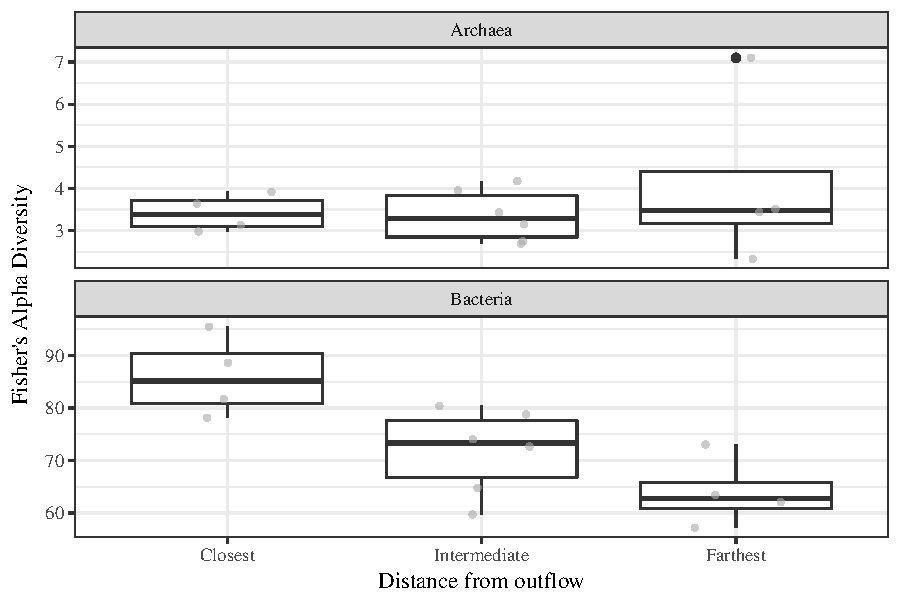
\includegraphics[width=\maxwidth]{figs/boxdivcont} 

}

\caption[Estimates of Fisher's alpha diversity for archaea and bacteria genera grouped by approximate distance from wastewater outflow pipes]{Estimates of Fisher's alpha diversity for archaea and bacteria genera grouped by approximate distance from wastewater outflow pipes. Alpha was was based on methods in Fisher et al. (1943) that measure diversity as a function of richness and abundance at a site.}\label{fig:boxdivcont}
\end{figure}


\end{knitrout}

% Table created by stargazer v.5.2 by Marek Hlavac, Harvard University. E-mail: hlavac at fas.harvard.edu
% Date and time: Fri, Nov 03, 2017 - 3:17:46 PM
\begin{table}[!htbp] \centering 
  \caption{Summary of analysis of variance results for bacteria and archaea diversity with distance from outflow.  Diversity measures were based on Fisher's Alpha (Fisher et al. 1943) using abundance of genera at each site. The model intercept is the average diversity estimate (standard error in parentheses) at all close sites and the remaining parameter estimates (intermediate and farthest) are referenced accordingly.} 
  \label{} 
\begin{tabular}{@{\extracolsep{5pt}}lcc} 
\\[-1.8ex]\hline 
\hline \\[-1.8ex] 
 & \multicolumn{2}{c}{Models} \\ 
\cline{2-3} 
 & Bacteria & Archaea \\ 
\hline \\[-1.8ex] 
 Constant (close) & 85.965$^{***}$ & 3.419$^{***}$ \\ 
  & (3.797) & (0.591) \\ 
  & & \\ 
 Intermediate & $-$14.252$^{**}$ & $-$0.061 \\ 
  & (4.902) & (0.763) \\ 
  & & \\ 
 Farthest & $-$22.048$^{***}$ & 0.678 \\ 
  & (5.369) & (0.836) \\ 
  & & \\ 
\hline \\[-1.8ex] 
Observations & 14 & 14 \\ 
R$^{2}$ & 0.614 & 0.087 \\ 
Adjusted R$^{2}$ & 0.544 & $-$0.079 \\ 
Residual Std. Error (df = 11) & 7.593 & 1.183 \\ 
F Statistic (df = 2; 11) & 8.740$^{***}$ & 0.524 \\ 
\hline 
\hline \\[-1.8ex] 
\textit{Note:}  & \multicolumn{2}{r}{$^{*}$p$<$0.1; $^{**}$p$<$0.05; $^{***}$p$<$0.01} \\ 
\end{tabular} 
\end{table} 


\end{document}
